\documentclass[12pt,letterpaper]{article}
\usepackage[utf8]{inputenc}                  
\usepackage[spanish]{babel}                  
\addto\captionsspanish{\renewcommand{\tablename}{Tabla}}		\addto\captionsspanish{\renewcommand{\listtablename}{Índice de tablas}}
\addto\captionsspanish{\renewcommand{\appendixpagename}{Apéndices}}
\addto\captionsspanish{\renewcommand{\appendixtocname}{Apéndices}}
\usepackage{geometry}                         
\geometry{left=18mm,right=18mm,top=21mm,bottom=21mm} 
\usepackage{ucs}
\usepackage{amsmath}      
\usepackage{amsfonts}     
\usepackage{amssymb}
\usepackage{graphicx}   
\usepackage[lofdepth,lotdepth]{subfig}	
\usepackage{unitsdef}	  
\usepackage{pdfpages}   
\usepackage[title, titletoc]{appendix} 
\renewcommand{\unitvaluesep}{\hspace*{4pt}}	
\usepackage[colorlinks=true,urlcolor=black,linkcolor=black,citecolor=black]{hyperref}     
\usepackage{float}	 
\usepackage{booktabs}
\batchmode
\pagestyle{plain} 
\pagenumbering{Roman} 
\usepackage{lastpage}
\usepackage{fancyhdr}
\pagestyle{fancy}		
\usepackage{amsmath}
\usepackage{listings}
\usepackage[newfloat]{minted}
\usepackage{caption}
\newenvironment{code}{\captionsetup{type=listing}}{}
\SetupFloatingEnvironment{listing}{name=\textbf{Código fuente}}
\setlength{\headheight}{16pt}


\usepackage{xurl}


% Document config
\usepackage{tikz}
\usepackage{url}


%%%%%%%%%%%%%%%%%%%%%%%%%%%%%%%%%%%%

\title{
{
    \begin{tikzpicture}[overlay, remember picture]
            \node[anchor=north west, %anchor is upper left corner of the graphic
                xshift=2cm, %shifting around
                yshift=-4cm] 
                at (current page.north west) %left upper corner of the page
            {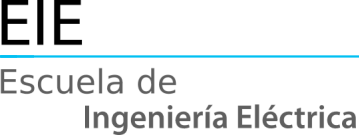
\includegraphics[height=1.3cm]{img/logoEIE.png}}; 
        \end{tikzpicture}
        \begin{tikzpicture}[overlay, remember picture]
            \node[anchor=north east, %anchor is upper left corner of the graphic
                xshift=-2cm, %shifting around
                yshift=-4cm] 
                at (current page.north east) %left upper corner of the page
            {
\includegraphics[height=1.3cm]{img/logoUCR.png}}; 
        \end{tikzpicture}
    \Large 
        %%%%%%%%%%%%%%%%% EDITAR PORTADA %%%%%%%%%%%%%%%%%%
        \textbf{Universidad de Costa Rica}\\
        Facultad de Ingeniería\\
        Escuela de Ingeniería Eléctrica\\
        \texttt{IE-0117} Programación Bajo Plataformas Abiertas\\~\\
        \vspace*{0.5cm}
    \LARGE \textbf{Proyecto Programación Bajo Plataformas Abiertas 
    }}
    ~\\~\\
    {\vspace*{1 in}}\Large Profesor: Andrés Mora Zuñiga\\ Grupo 03\vspace*{1 in}
}
\author{Alexis Rodriguez Romero - \texttt{B-96729} \\
Rodrigo López Soto - \texttt{B-23776}\\
Joselyn Barquero Castillo - \texttt{B-88858} \\
Noel Blandon Saborio - \texttt{B-61097}}

\date{\vspace*{2in}II Ciclo-2020}

%%%%%%%%%%%%%%% EDITAR ENCABEZADOS %%%%%%%%%%%%%%%%%
\lhead{IE-0117 Programación Bajo Plataformas Abiertas}
\chead{}
\rhead{}
\lfoot{Escuela de Ingeniería Eléctrica}
\cfoot{\thepage}
\rfoot{Universidad de Costa Rica}


\begin{document}

\pdfbookmark[1]{Portada}{portada} 	% Marcador para el título

\clearpage\maketitle   % Título

\newpage 
\setcounter{page}{2}
\tableofcontents
\newpage
% \listoffigures
% \listoftables

\newpage
\pagenumbering{arabic}


%%%%%%%%%%%%%%%%% AQUÍ EMPIEZA EL DOCUMENTO %%%%%%%%%%%




\section{Introducción} 
En este proyecto se pretende realizar un juego de naves espaciales en el lenguaje de programación Python mediante el uso de la librería Pygame, el juego consiste en una serie de niveles en los cuales el jugador se enfrenta a naves enemigas mediante una interfaz gráfica el jugador tiene control de la nave la cual se puede desplazar horizontal y verticalmente el usuario cuenta con una serie de armas y límite de vidas para enfrentarse a las naves enemigas las cuales cuentan con movimiento vertical y horizontal el usuario pierde cuando las naves contrarias lo impactan directamente. Además se incluirán distintas pistas musicales para cada nivel así como un menú principal donde el usuario pueda personalizar aspectos referentes a su partida tales como nombre de usuario color de la nave y tipos de armas, finalmente el juego guardara mediante un sistema de puntos el avance de cada jugador para poder incrementar la rivalidad entre distintos usuarios. 

El juego se programará haciendo uso del \textit{framework} de Python para videojuegos llamado \textit{Pygame}, con el cual se facilita la programación de todas las herramientas relativas al videojuego porque tiene funciones y métodos ya construidos para utilizarse en este contexto.



\section{Justificación} 
El proyecto pretende utilizar el conocimiento del curso Programación Bajo Plataformas Abiertas. Por esta razón la realización de un videojuego bajo la filosofía de software libre permitirá a otras personas hacer uso del videojuego para ocio y estudiar el código para así poder modificar aspectos que deseen o estudiar el algoritmo bajo el cuel funciona este. 

El videojuego permite así estudiar las herramientas de \textit{Pygame} y compartirla con otras personas interesadas para que lo jueguen, estudien y si así se desea que lo modifiquen,  de esta manera siguiendo la filosofía de \textit{software libre} en plataformas abiertas.


 
\section{Alcances}
En este sentido el juego se pretende que se pueda ejecutar en plataforma de escritorio, particularmente en sistema operativo Linux (se probará con las distribuciones Ubuntu  Debian). Para otras plataformas como Windows o plataformas mívoles como Android o iOS no se pretende probar, sin embargo esto podría hacerse como trabajo futuro. 

Las características modificables serán el color de las naves, las pistas musicales y la cantidad de vidas. Todo esto utilizando \textit{Pygame} por lo que la ejecución del juego estará restringida a computadoras de escritorio con sistema operativo Linux y con \textit{Pygame} debidamente instalado.

Como trabajo futuro se pueden agregar distintos tipos de escenarios, diferentes tipos de naves (aliadas y enemigas), diferentes tipos de armas, entre otros, todo configurable desde el menú principal. 


\section{Objetivos} 
\subsection{Objetivo general}
Realizar un juego de naves espaciales en el lenguaje de programación Python mediante el uso de la librería pygame, el juego consiste en una serie de niveles en los cuales el jugador se enfrenta a naves enemigas, mediante una interfaz gráfica el jugador tiene control de la nave la cual se puede desplazar horizontal y verticalmente mediante el uso del teclado.


\subsection{Objetivos específicos} 
\begin{enumerate}
    \item  Investigar características y herramientas de la librería Pygame de Python.
        \begin{itemize}
            \item Entregable 1: Realizar un resumen que muestre las principales características y herramientas que ofrece la librería Pygame. 
            
        \end{itemize}

    \item  Programar una función principal del juego naves especial. 
        \begin{itemize}
            \item Entregable 2: Entrega del código correspondiente a la función principal del juego verificar funcionalidad. 
            
        \end{itemize}
   
    \item  Programar una función que permita crear el objeto (nave espacial) además de implementar el movimiento de la misma.  
        \begin{itemize}
            \item Entregable 3: Entrega del código correspondiente a  las funciones de crear el objeto que incluye dimensiones colores y formas a su vez una función que permita el movimiento del objeto por medio de coordenadas verificar funcionalidad. 
            
        \end{itemize}
        
    \item  Programar función que adhiera armas (lazers) al objeto además de aplicar restricciones del movimiento al objeto.
    
 
        \begin{itemize}
            \item Entregable 4: Entrega del código correspondiente a  las funciones de armas de la nave y restricciones de movimiento.

            
        \end{itemize}
        
    \item  Programar función que permita incluir distintos niveles al juego con distintas configuraciones de enemigos.  
    
 
        \begin{itemize}
            \item Entregable 5: Entrega del código correspondiente a  la función de niveles con un total de 3 niveles con distintas configuraciones de enemigos.  

            
        \end{itemize}
        
    \item  Programar función que permita incluir distintas pistas musicales a cada uno de los niveles del juego.   
    
 
        \begin{itemize}
            \item Entregable 6: Entrega del código correspondiente a  la función sonidos la cual incluye tres pistas para cada uno de los niveles. 

            
        \end{itemize}
        
    \item Diseñar y programar una  función que adhiera un menú interactivo para el usuario.   
    
 
        \begin{itemize}
            \item Entregable 7: Entrega del código correspondiente a  la función menú la cual incluye opciones como iniciar o salir del juego. 

            
        \end{itemize}
    
    \item Diseñar y programar una función que permita guardar el avance de las distintas partidas realizadas en el juego. 
 
        \begin{itemize}
            \item Entregable 8: Entrega del código correspondiente a  la función puntos la cual permite guardar el avance de cada uno de los jugadores. 

            
        \end{itemize}
        
\end{enumerate}

  
 \section{Metodología} 
 El lenguaje de programación principal para la elaboración del proyecto es Python, con el uso de Pygame que corresponde a un conjuto de módulos del lenguaje de programación en conjunto con la librería SDL (acrónimo de Simple DirectMedia Layer). \vspace{5mm}\\
 \indent SDL es una biblioteca de desarrollo multiplataforma diseñada para proporcionar acceso de bajo nivel a hardware de audio, teclado, mouse, joystick y gráficos a través de OpenGL y Direct3D. Es compatible con Windows, Mac OS X, Linux, iOS, Android, además para otras plataformas se puede encontrar soporte en el código fuente.
\vspace{5mm} \\
\indent OpenGL es una API (Application Programming Interface) de gráficos 2D y 3D que permite crear aplicaciones de software de gráficos de alto rendimiento y visualmente atractivas. Con ayuda de la biblioteca SDL y Pygame será posible la creación del juego de naves añandiendo contenido multimedia y figuras en 2D. \vspace{5mm} \\
\indent Como referencias bibliográficas para la realización del juego se estará consultando la página oficial de Pygame, donde se encuentra una gran documentación que describe los posibles módulos a utilizar. Así bien, también, se investigará en foros y en distintas páginas web, que permitan resolver dudas que surgan en la realización del mismo, y complementen de manera satisfactoria la teoría expuesta.



  
\section{Marco Teórico} 
Para el presente marco teórico, se presentará la historia y atributos del lenguaje de programación a utilizar. Trabajaremos con una plataforma de programación open source. Por ello es importante definir que es un código abierto. En la revista \textit{Acceso Abierto y Software Libre}, escrita por Manuel Alejandro Echeverría, explica que el código abierto es un modelo de desarrollo de software basado en la colaboración abierta. Empezado en 1983 por Richard Stallman con la meta de difundir un sistema eficaz compatible con Unix, que fuese de código abierto donde cualquiera pueda utilizarlo, modificarlo y adaptarlo a sus necesidades. Echeverría aclara que la percepción bajo la noción de código open-source es sencilla: cuando los programadores pueden analizar, arreglar y redistribuir el código ``original'' de un programa, este evoluciona, se desarrolla y mejora. Los usuarios lo adaptan a sus necesidades, corrigen sus errores en un menor periodo a la aplicada en el proceso de programación convencional, dando como resultado la fabricación de un mejor software.\vspace{5mm}\\
\indent Como recalcan los autores de Ciencias Holguín, el lenguaje de programación Python o cualquier otro lenguaje de programación son la herramienta básica de construcción de programas, como lo son el machete y el azadón para un campesino, el pico y la pala para un constructor. Por ello y lo ventaja resaltada anteriormente de las plataformas open-source, se escogió trabajar en el lenguaje de Python ya que este posee una licencia de código abierto, denominada Python Software Foundation License. Este fue creado en la década de los 80 por el programador de origen holandés llamado Guido van Rossum. Se trata de un lenguaje de programación multiparadigma, ya que soporta orientación a objetos, programación imperativa y, en menor medida, programación funcional. Es un lenguaje interpretado, dinámico y multiplataforma. Fue diseñado para ser leído con facilidad ya que una de sus principales características es el uso de palabras donde otros lenguajes utilizarían símbolos. Ejemplo, los operadores lógicos !, || y \&\& en Python se escriben not, or y and, respectivamente. Además cuenta con una amplia variedad de bibliotecas disponibles y compatibilidad con librerías de otras plataformas como c y c++. Se podría decir que Python es más fácil de aprender que otros lenguajes como c, esto sumo un peso más a la hora de elegirlo.\vspace{5mm}\\
\indent Para este proyecto de programación, nos enfocaremos en el módulo de Pygame, basado en una biblioteca llamada SDL. Permitiéndole a Python crear juegos y programas multimedia. Se toma en cuenta que este es modular, portátil, con absoluto orden y control en el archivo principal utilizando funciones. Características fundamentales que tienen mucho peso en un primer proyecto grupal de programación, dado que se hace más sencillo distribuir el trabajo entre los participantes.\vspace{5mm}\\
\indent Python es un lenjuaje de programción interpretado, orientado a objetos y de alto nivel con semántica dinámica. Sus estructuras de datos integradas de alto nivel, combinadas con tipado dinámico y enlace dinámico, lo hacen muy atractivo para el desarrollo rápido de aplicaciones, así como para su uso como lenguaje de scripts o como pegamento para conectar componentes existentes. La sintaxis simple y fácil de aprender de Python enfatiza la legibilidad y por lo tanto reduce el costo de mantenimiento del programa. Python admite módulos y paquetes, lo que fomenta la modularidad del programa y la reutilización del código. El intérprete de Python y la extensa biblioteca estándar están disponibles en formato fuente o binario sin cargo para todas las plataformas principales y se pueden distribuir libremente.\vspace{5mm} \\
\indent Pygame es una biblioteca multimedia de Python para crear juegos y aplicaciones multimedia. Es un wrapper de la biblioteca SDL (Simple DirectMedia Layer). Pygame es gratis. Publicado bajo la licencia LGPL (Library General Public License), puede crear juegos de código abierto, freeware, shareware y comerciales con él. \vspace{5mm} \\
\indent Como se meciona en el anterior aparatado, SDL es una biblioteca de desarrollo multiplataforma diseñada para proporcionar acceso de bajo nivel a hardware de audio, teclado, mouse, joystick y gráficos a través de OpenGL y Direct3D. A su vez OpenGL es una API (Application Programming Interface) de gráficos 2D y 3D que permite crear aplicaciones de software de gráficos de alto rendimiento y visualmente atractivas.\vspace{5mm} \\
\indent A continuación se presenta una descripción general de los módulos en Pygame, que serán de utilidad en la realización del proyecto.
\begin{itemize}
    \item cdrom: reproducción
    \item cursors: cargar imágenes de cursor, incluye cursores estándar
    \item display: controlar la ventana de visualización o la pantalla
    \item draw: dibujar formas simples en una superficie
    \item event: administrar eventos y la cola de eventos
    \item font: crear y renderizar fuentes TrueType
    \item image: guardar y cargar imágenes
    \item joystick: administrar dispositivos de joystick
    \item key: administrar el teclado
    \item mouse: administrar el mouse
    \item sndarray: manipular sonidos con numpy
    \item surfarray: manipular imágenes con numpy
    \item time: tiempo de control
    \item transform: escalar, rotar y voltear imágenes

\end{itemize}

NumPy es el paquete fundamental para la computación científica en Python. Es una biblioteca de Python que proporciona un objeto de matriz multidimensional, varios objetos derivados (como matrices y masked arrays) y una variedad de rutinas para operaciones rápidas en matrices, que incluyen manipulación matemática, lógica, de formas, clasificación, selección, transformadas discretas de Fourier, álgebra lineal básica, operaciones estadísticas básicas, simulación aleatoria.\vspace{5mm}\\
\indent En el núcleo del paquete NumPy, está el objeto ndarray . Esto encapsula matrices n- dimensionales de tipos de datos homogéneos, con muchas operaciones que se realizan en código compilado para el rendimiento.


 \section{Estado de la Cuestión} 
En 1979 se introduce el precursor del estilo de juego de naves espaciales a manos de Namco, nombrado como Galaga. En este el jugador controla una nave que debe resistir y enfrentarse a una oleada de aliens que atacan disparando bombas y actuando como kamikazes. El juego tiene un dificultad escalonada, pero en sí sus enemigos y armas son muy similares. Las primeras versiones solo cuentan con un movimiento horizontal y no vertical. Cabe recalcar que este juego es licenciado, entonces la compañía espera en las versiones gratuitas de nueva generación, implementar anuncios dentro del juego o inclusión de micro-transacciones. En el caso que el juego no esté gratuito, no existe otra forma que comprarlo para poder disfrutarlo. Como punto positivo es que está en la mayoría de las plataformas de entretenimiento creadas hasta ahora. En nuestro caso queremos realizar un tipo de juego similar a este pero que sea totalmente abierto y así poder modernizar ciertas mecánicas del original. Por ejemplo, un menú principal más amigable con el usuario y que permita personalizar aspectos referentes a la partida, que en el juego original de namco no se logra hacer. Además de la inclusión del movimiento vertical.
\vspace{5mm}\\
\indent Si se compara a Python con otros lenguajes de programación se tiene, por ejemplo en Python no hay necesidad de punto y coma y llaves en el programa en comparación con Java, que mostrará un error de sintaxis si se olvidó agregar llaves o punto y coma en el programa. El código Python por lo general requiere menos líneas de código en comparación con Java para escribir el mismo programa. Python se escribe dinámicamente, lo que significa que uno solo tiene que asignar un valor a una variable en tiempo de ejecución, el intérprete de Python detectará el tipo de datos en sí mismo en comparación con Java, donde uno tiene que mencionar explícitamente el tipo de datos. \vspace{5mm}\\
\indent Python admite varios tipos de modelos de programación, como programación imperativa, orientada a objetos y de procedimientos, en comparación con Java, que se basa completamente en modelos de programación basados en objetos y clases.
Python es fácil de leer y aprender, lo cual es beneficioso para los principiantes que esperan comprender los fundamentos de la programación rápidamente en comparación con Java, que tiene una curva de aprendizaje pronunciada debido a sus sintaxis complejas predefinidas.
La sintaxis concisa de Python lo convierte en una mejor opción para las personas de otras disciplinas que desean utilizar el lenguaje de programación para la minería de datos, el procesamiento neuronal, el aprendizaje automático o el análisis estadístico en comparación con la sintaxis de Java, que es larga y difícil de leer.
\vspace{5mm}\\
\indent Si se compara con C++, Python es más eficiente en memoria debido a su recolección automática de garbage en comparación con C ++ que no admite la recolección de basura.
El código Python es fácil de aprender, usar y escribir en comparación con C ++, que es difícil de entender y usar debido a su compleja sintaxis.\vspace{5mm}\\
\indent Python utiliza un intérprete para ejecutar el código, lo que facilita su ejecución en casi todas las computadoras o sistemas operativos. en comparación con el código C ++ que no se ejecuta en otras computadoras hasta que se compila en esa computadora.\vspace{5mm}\\
\indent Python puede usarse fácilmente para el desarrollo rápido de aplicaciones debido a su tamaño de código más pequeño en comparación con C ++, que es imposible de usar para el desarrollo rápido de aplicaciones debido a sus grandes fragmentos de código.
La legibilidad del código Python es más, ya que se parece al inglés real en comparación con el código C ++ que contiene estructuras y sintaxis difíciles de leer. \vspace{5mm}\\
\indent Las variables definidas en Python son fácilmente accesibles fuera del ciclo en comparación con C ++ en el que el alcance de las variables está limitado dentro del ciclo. \vspace{5mm}\\
\indent Existen también alternativas de código abierto, tales como Godot, Godot Engine es un motor de juegos multiplataforma para crear juegos en 2D y 3D desde una interfaz unificada. Proporciona un conjunto completo de herramientas comunes, para que los usuarios puedan concentrarse en crear juegos sin tener que reinventar algo que ya existe. Los juegos se pueden exportar con un clic a varias plataformas, incluidas las principales plataformas de escritorio (Linux, macOS, Windows), así como plataformas móviles (Android, iOS) y basadas en la web (HTML5).
\vspace{5mm}\\
\indent Godot es completamente gratuito y de código abierto bajo la licencia permisiva del MIT. Los juegos de los usuarios son suyos, hasta la última línea del código del motor. El desarrollo de Godot es totalmente independiente y está impulsado por la comunidad, lo que permite a los usuarios ayudar a dar forma a su motor para que coincida con sus expectativas.
\vspace{5mm}\\
\indent Uno de los juegos más completos de naves en Python, se puede encontrar en el sistema de gestión de proyectos y control de versiones de código, GitHub (Referencia bibliográfica 5). Este nos permite elegir la nave con la cual queremos jugar y cuenta con diferentes fases. Cuenta hasta con una jefe final. En el apartado del diseño puede observarse que, es un proyecto que lleva mucho detrás. Pero debido a su antigüedad el autor no depuró ciertos errores. Al descargarlo hay que modificar ciertos directorios para que el juego inicie sin problemas, también por mencionarse, la música y ciertos elementos son repetitivos.\vspace{5mm}\\
\indent Comparando esta versión con el proyecto propuesto, se espera que el usuario logre disfrutar sin tener los inconvenientes de los directorios. Además de tener una mejor personalización de las naves y una mejora en la implementación de la banda sonora. También se observó que ciertas colisiones resultan deficientes, dando como resultado una mala experiencia de juego, mencionando también que, la nave solo cuenta con un movimiento tipo horizontal, un referente a mejorar en nuestra versión, añadiendo una mejor detección de colisiones y una correcta implementación de movimiento. 


  
\section{Cronograma} 
 En la siguiente figura se muestra el cronograma de actividades.  
\begin{figure}[H]
\centering
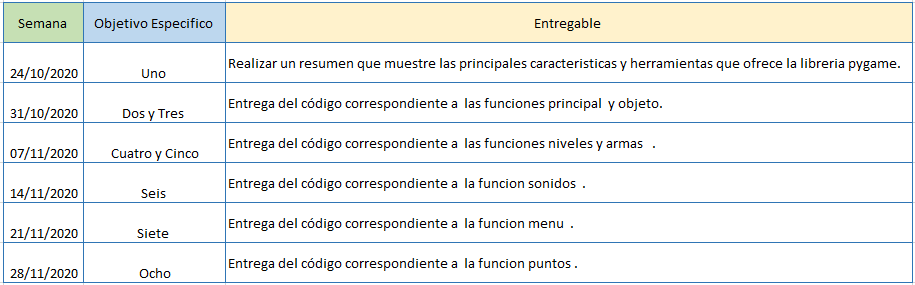
\includegraphics[width=16cm]{cronograma.PNG}
\caption{Cronograma}
\end{figure}


\subsection{Diagrama de Gantt} 
En la siguiente figura se muestra el diagrama de Gantt, una herramienta importante para el orden y desarrollo de las actividades del proyecto, con este diagrama se puede verificar el cumplimiento de las asignaciones, así como fechas tentativas para la realización de cada una de las actividades.
\begin{figure}[H]
\centering
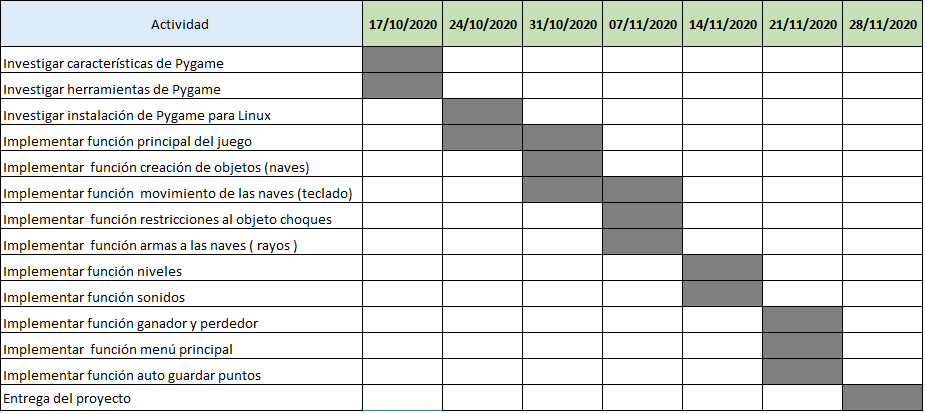
\includegraphics[width=16cm]{Gannt.PNG}
\caption{Diagrama de Gantt}
\end{figure}


\section{Diseño}

\begin{figure}[H]
\centering
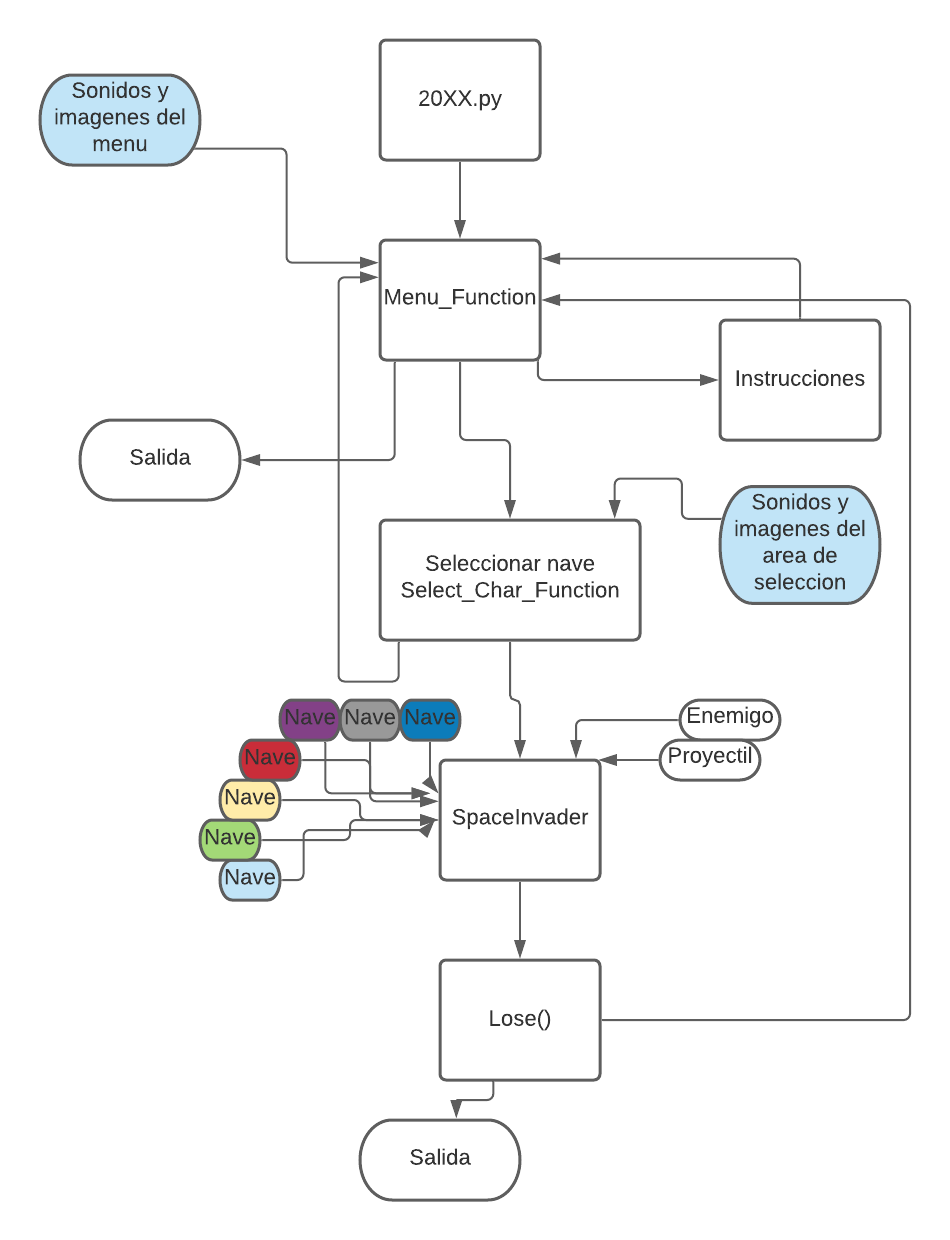
\includegraphics[width=16cm]{Blank diagram.png}
\caption{Diagrama de Flujo}
\end{figure}
Para el diseño del proyecto se siguió el esquema planteado en diagrama de la figura 3. Se parte de un "Main" llamado 20XX.py del cual se referencia una función menú. En estas se implementaron mediante biblioteca pygame, sonidos y imágenes para darle vida al menú, asi cumpliendo con uno de los primeros objetivos planteados.
\vspace{5mm}\\
\indent Este Menu da como opciones, salirse del juego, leer las instrucciones para jugar y después regresar al menú anterior, por ultimo ejecutar la funcion Select\_Char\_Function. En esta Función se vuelve importar ciertos sonidos e imágenes que se van a utilizar en la pantalla de selección de naves, esta función tiene unos condicionales que si se da la elección de "x" nave esta importa el nombre y la dificultad correspondiente a la siguiente función. Si no se puede devolver a la función del menú anterior.\vspace{5mm}\\
\indent Ejecutada la función SpaceInvader se procede a llamar la función de las naves con el parámetro del nombre obtenido con la función anterior. Además se procede a llamar a los enemigo y proyectiles con una variable de rapidez editable, esta varia según la dificultad que tiene cada nave. Al Final de esta función se llama una función Lose() que requiere el nombre de la nave y su puntuación. Para al final compartirnos nuestro puntaje acompañado de dos opciones, Jugar de nuevo y Salir. Una se devuelve al menu y la otra cierra la ventana 


\section{Diseño e implementación}
\subsection{Objetivo 1}
\subsubsection{Instalación de Pygame}
Para la instalación de Pygame en Linux, basta usar el siguiente comando en terminal \texttt{sudo apt-get install python-pygame}. Para la instalación en Windows, desde el command prompt se utiliza el siguiente comando \texttt{pip install pygame}, para una versión mas reciente de Python, como la 3.9, el siguiente comando funciona en la instalación \texttt{pip3 install pygame --only-binary :all:}.

\subsection{Objetivo 2}
\subsubsection{Desplegar una ventana en Python} \label{objetivo2}
 Como se observa en el código \ref{entregable1}, se importa el módulo \texttt{sys}, este proporciona acceso a algunas variables utilizadas o mantenidas por el intérprete y acceso a funciones que interactúan fuertemente con el intérprete. Por ejemplo, en el código se utiliza para cerrar la ventana creada.\vspace{5mm}\\
\indent Antes de hacer uso de los módulos de Pygame, se debe utilizar \texttt{pygame.init()} para inicializar todos los módulos importados anteriormente.\vspace{5mm}\\
\indent\texttt{Display} es un módulo de pygame para controlar la ventana de visualización y la pantalla. Con este módulo se crea la nueva ventana.
\begin{listing}[H]
\begin{minted}{python}
import pygame, sys
from pygame.locals import *

pygame.init()
ventana = pygame.display.set_mode((400, 300))

pygame.display.set_caption("Proyecto plataformas")

while True:
    for evento in pygame.event.get():
        if evento.type == QUIT:
            pygame.quit()
            sys.exit()

    pygame.display.update()

\end{minted}
\caption{Desplegar una ventana en Python}
\label{entregable1}
\end{listing}

\subsection{Objetivo 3}
\subsubsection{Creación y movimiento de la nave} \label{objetivo3}
Como se observa en el código \ref{entregable2}, para la creación de objetos en el juego, se escribe una clase para cada tipo de objeto, en este caso, la nave espacial, donde se implementan las funciones de la misma. En la función \texttt{\_\_init\_\_} se definen los atributos de la nave, por ejemplo, donde se va a colocar en la ventana anteriormente creada.\vspace{5mm}\\
\indent En la función \texttt{movimiento}, se define qué tan a la izquierda o a la derecha de la ventana puede llegar la nave, de acuerdo con el ancho establecido.\vspace{5mm}\\
\indent Para este objetivo se establece la función \texttt{disparar}, mas aun no se trabaja en ella, solamente imprime en terminal.
En la función \texttt{dibujar}, se utiliza \texttt{superficie.blit()} para dibujar la nave sobre el fondo, recibe los argumentos del objeto a dibujar y el destino. 
\begin{listing}[H]
\begin{minted}{python}
class naveEspacial(pygame.sprite.Sprite):
    def __init__(self):
        pygame.sprite.Sprite.__init__(self)
        self.ImagenNave = pygame.image.load("Imagenes/nave.jpg")
        self.rect = self.ImagenNave.get_rect()
        self.rect.centerx = ancho/2
        self.rect.centery = alto - 30

        self.listaDisparo = []
        self.Vida = True
        self.velocidad = 20
        
    def movimiento(self):
        if self.Vida == True:
            if self.rect.left <= 0:
                self.rect.left = 0
            elif self.rect.right > 870:
                self.rect.right = 840
                
    def disparar(self):
        print ("Disparo")

    def dibujar(self, superficie):
        superficie.blit(self.ImagenNave,self.rect)    

\end{minted}
\caption{Creación y movimiento de la nave}
\label{entregable2}
\end{listing}

En la función principal \texttt{SapceInvader()} se utiliza el módulo para trabajar con el teclado, se establecen las teclas con las que se mueve la nave y con la que dispara, como se observa en el código \ref{entregable21}.

\begin{listing}[H]
\begin{minted}{python}
def SpaceInvader():
    pygame.init()
    ventana =pygame.display.set_mode((ancho,alto))
    pygame.display.set_caption("Space Invader")
    ImagenFondo = pygame.image.load("Imagenes/Fondo.jpg")
    jugador = naveEspacial()
    enJuego = True

    while True:

        jugador.movimiento()
        for evento in pygame.event.get():
            if evento.type ==QUIT:
                pygame.quit()
                sys.exit()

            if enJuego == True:
                if evento.type ==pygame.KEYDOWN:
                    if evento.key == K_LEFT:
                        jugador.rect.left -= jugador.velocidad
                    elif evento.key == K_RIGHT:
                        jugador.rect.right += jugador.velocidad
                    elif evento.key == K_s:
                        jugador.disparar()
        ventana.blit(ImagenFondo,(0,0))
        jugador.dibujar(ventana)        
        pygame.display.update()

SpaceInvader()
\end{minted}
\caption{Implementación del módulo de pygame .key para el movimiento de la nave}
\label{entregable21}

\end{listing}


\subsection{Objetivo 4} 
\subsubsection{Creación de la clase proyectil} \label{objetivo4}
Esta clase se desarrolla de manera similar a la clase de nave explicada anteriormente. Como se puede observar en el código \ref{objetivo41}, en la función \texttt{\_\_init\_\_} se definen los atributos del láser, colocándose en la misma posición de la nave (los argumentos se definen en la función principal). En la función \texttt{trayectoria} se desea que el láser vaya en la posición Y. \vspace{5mm}\\
\indent En la función principal se crea el objeto que corresponde al láser que envía la nave del jugador. 
Se crea una lista disparo en la clase nave, además, en la función disparar, la lista recibe el objeto del láser creado en la función principal.

\begin{listing}[H]
\begin{minted}{python}
class Proyectil(pygame.sprite.Sprite):
    def __init__(self, posx, posy):
        pygame.sprite.Sprite.__init__(self)
        self.imagenProyectil = pygame.image.load("Imagenes/disparoa.jpg")
        self.rect = self.imagenProyectil.get_rect()
        self.velocidadDisparo = 5
        self.rect.top = posy
        self.rect.left = posx
        
    def trayectoria(self):
        self.rect.top = self.rect.top -self.velocidadDisparo

    def dibujar(self, superficie):
        superficie.blit(self.imagenProyectil, self.rect)
\end{minted}
\caption{Creación de la clase proyectil}
\label{objetivo41}

\end{listing}

\subsection{Objetivo 5} \label{objetivo5}
Para la configuración de los diferentes niveles de dificultad se consideraron dos factores:
\begin{itemize}
    \item La cantidad de enemigos
    \item El tiempo promedio entre disparos
\end{itemize}

De esta manera los niveles más difíciles tendrán más enemigos que disparan más rápidamente. Particularmente la variable \textbf{self.rangodisparo}.   de la función \textbf{\_init\_} define un límite sobre el cual se evaluarán números aleatorios entre 0 y 99 y se compararám con \textbf{self.rangodisparo}, si el número aleatorio es menor a \textbf{self.rangodisparo} ocurre un disparo por parte de la nave enemiga, y si es mayor no dispara, de manera que para valores más grandes de \textbf{self.rangodisparo} los disparos ocurren con mayor frecuencia y la dificultad es aumentada en consecuencia. Esto se logra porque la función \textbf{\_ataque} llama a la función \textbf{\_disparo} (de la clase Invasor) únicamente cuando el número aleatorio generado es menor que el valor constante definido por  \textbf{self.rangodisparo}, tal como se muestra en el Código fuente\ref{ataque}.


\begin{listing}[H]
\begin{minted}{python}
    def __ataque(self):
        if(randint(0,100)<self.rangoDisparo):
            self.__disparo()
    def __disparo(self):
        x,y = self.rect.center
        miProyectil=Proyectil.Proyectil(x,y,"Imagenes/disparob.jpg", False)
        self.listaDisparo.append(miProyectil)
\end{minted}
\caption{Implementación de la función ataque}
\label{ataque}
\end{listing}
Así mismo, la cantidad de enemigos tiene que ver con la cantidad de enemigos que se adjunten al arreglo \textbf{listaEnemigo} desde la función \textbf{CargarEnemigos}. De este modo los niveles más difíciles tendrán más cantidad de enemigos y los más fáciles menos, tal como se muestra en el Código fuente\ref{cargarenem}. 


        
    \begin{listing}[H]
\begin{minted}{python}
def cargarEnemigos(): 
    posx = 100
    for x in range(1,5+Dificultad):
        enemigo = Enemigo(posx,100,40, "Imagenes/marcianoA.jpg",
        "Imagenes/MarcianoB.jpg",Dificultad)
        listaEnemigo.append(enemigo)
        posx = posx+200
    
    posx = 100
    for x in range(1,5+Dificultad):
        enemigo2 = Enemigo(posx,0,40, "Imagenes/Marciano2A.jpg",
        "Imagenes/Marciano2B.jpg",Dificultad)
        listaEnemigo.append(enemigo2)
        posx = posx+200

    posx = 100
    for x in range(1,5+Dificultad):
        enemigo3 = Enemigo(posx,-100,40, "Imagenes/Marciano3A.jpg",
        "Imagenes/Marciano3B.jpg", Dificultad)
        listaEnemigo.append(enemigo3)
        posx = posx + 200
\end{minted}
\caption{Implementación de la función CargarEnemigos}
\label{cargarenem}
\end{listing}
\subsection{Objetivo 6} \label{objetivo6}
Para cumplir con el objetivo de las pistas musicales de fondo se utilizaron funciones de \textit{Pygame} que permiten añadir música de fondo y sonidos activados por eventos (como la colisión de una nave con una enemiga o con un disparo). Para cargar la música de fondo se utiliza la función \textbf{pygame.mixer.music.load}, a la cual se le introduce como parámetro un string que contiene la ruta de la pista que se reproducirá de fondo, la cual para este caso se utilizó en formato .mp3, la cual puede variar dependiendo de la dificultad. Así mismo, al inicio del juego se reproduce esta pista que se especificó mediante la función \textbf{pygame.mixer.music.play} la cual tiene como argumento la cantidad de veces que se reproducirá la pista. En el Código Fuente \ref{music} se muestra la manera en la que se realizó. Es importante mencionar que se definen tres rutas diferentes en el array Soundtrack, una diferente para cada nivel de dificultad.

\begin{listing}[H]
\begin{minted}{python}
    Soundtrack = ["Sonidos/Soundtrack.mp3", "Sonidos/Moonlight.mp3", "Sonidos/Fly.mp3"]
    pygame.mixer.music.load(Soundtrack[Dificultad])  #Definir ruta
    pygame.mixer.music.play(3)
\end{minted}
\caption{Forma en la que se agregó la música de fondo}
\label{music}
\end{listing}

Así mismo, para los sonidos activados por eventos se consideraron como eventos de activación la colisión entre naves, los disparos y la colisión de naves con disparos. En la clase Nave se definen las variables \textbf{self.sonidoDisparo} y \textbf{self.sonidoExplosion} que utilizan la función \textbf{pygame.mixer.Sound('ruta')} que define la ruta en la cual el juego buscará cada uno de los sonidos, de la manera mostrada en el código fuente \ref{disparosruta}.
Para este caso es importante mencionar que el formato que se utilizó es .wav, dado que \textit{Pygame} no permite reproducir dos pistas en formato .mp3 al mismo tiempo, de manera que para que no interfiera con la música de fondo se utilizó formato .wav. En las funciones \textbf{disparar()} y  \textbf{destruccion()} se reproducen los sonidos de disparo y explosión, respectivamente, de la manera mostrada en el código fuente \ref{disparos}. 


\begin{listing}[H]
\begin{minted}{python}
    def __init__(self, ancho, alto):
        pygame.sprite.Sprite.__init__(self)
        self.ImagenNave = pygame.image.load("Imagenes/nave.png")
        self.ImagenExplosion = pygame.image.load("Imagenes/explosion.jpg")
        self.rect = self.ImagenNave.get_rect()
        self.rect.centerx = ancho/2
        self.rect.centery = alto - 30
        self.listaDisparo = []
        self.Vida = True
        self.velocidad = 20
        self.sonidoDisparo = pygame.mixer.Sound("Sonidos/Disparo1.wav")  #Definir ruta, tiene que ser .wav
        self.sonidoExplosion = pygame.mixer.Sound("Sonidos/Disparo2.wav")n
\end{minted}
\caption{Forma en la que se agregó la ruta del sonido de los disparos}
\label{disparosruta}
\end{listing}

\begin{listing}[H]
\begin{minted}{python}
    def disparar(self,x,y):

        miProyectil = Proyectil.Proyectil(x,y, "Imagenes/disparoa.jpg", True)
        self.listaDisparo.append(miProyectil)
        self.sonidoDisparo.play()

    def destruccion(self):
        self.sonidoExplosion.play()
        self.Vida = False
        self.velocidad = 0
        self.ImagenNave = self.ImagenExplosion
\end{minted}
\caption{Forma en la que se reprodujo el sonido de los disparos}
\label{disparos}
\end{listing}

\subsection{Objetivo 7} \label{objetivo7} 
Retornando la posicion del mouse a cada momento con pygame.mouse.get\_pos\(\) al posicionarse encima del area de un sprite, detecta si recibio una pulsacion con mouse\_click en el area reservada. Esto lo consigue mediante condicionales, como se logra notar a continuación. Cabe mencionar que cada sprite tiene una función que se ejecuta si es pulsado por el mouse. Dando la posibilidad de elegir entre varias opciones

\begin{listing}[H]
\begin{minted}{python}
    if 174<mouse[0]<274 and 290<mouse[1]<340:
        screen.blit(play1,[174,290])
        screen.blit(instructionsbutton,[174,360])
    if 174<mouse[0]<274 and 360<mouse[1]<410:
        screen.blit(instructionsbutton1,[174,360])
    if 174<mouse_click[0]<274 and 360<mouse_click[1]<410:
        click.play()
        instructions(highscore)
        break
    if 174<mouse_click[0]<274 and 290<mouse_click[1]<340:
        click.play()
        select_ship(highscore)
        break
    screen.blit(quitbutton,[174,430])
    if 174<mouse[0]<274 and 430<mouse[1]<480:
        screen.blit(quitbutton1,[174,430])
    if 174<mouse_click[0]<274 and 430<mouse_click[1]<480:
        pygame.quit()
        break
\end{minted}
\caption{Forma en la que trabajo el menú}


\label{menu}
\end{listing}






\subsection{Objetivo 8} \label{objetivo8}
Esta función es simple ya que desde el inicio se implemento en el archivo del juego un sistema de puntos. La función "Lose.py" lo que hace es solicitar del juego la puntuación obtenida y el nombre de la nave para anotarlo en la pantalla y en un archivo ".txt".


\begin{listing}[H]
\begin{minted}{python}
    f=open("Highscores.txt","a")
    f.write(ship_type.upper())
    f.write(" - ")
    f.write(str(score))
    f.write("\n")
    f.close()
    main_menu(highscore)
    break
\end{minted}
\caption{Forma en la que escribio los puntajes}


\label{menu}
\end{listing}
\newpage

\section{Validación}

\subsection{Sobre la implemetación \ref{objetivo2}}
Como se observa en la figura \ref{validacion102}, se logra desplegar una ventana que corrobora la implemetación \ref{objetivo2}.
\begin{figure}[H]
    \centering
    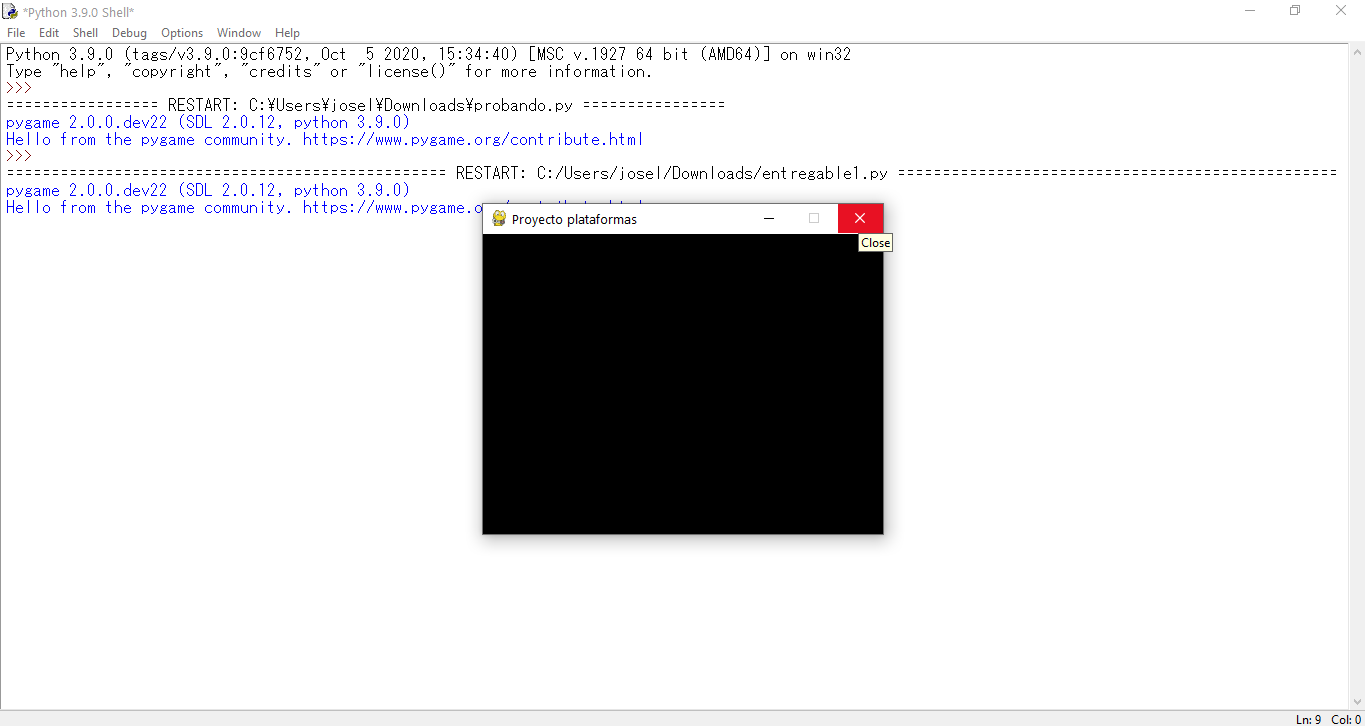
\includegraphics[width=0.7\linewidth]{validacion102.png}
    \caption{Validación de la implemetación \ref{objetivo2}}
    \label{validacion102}
\end{figure}

\subsection{Sobre la implementación \ref{objetivo3}}
Como se observa en la figura \ref{validacion01}, se corrobora la funcionalidad de la implementación \ref{objetivo3}.
\begin{figure}[H]
    \centering
    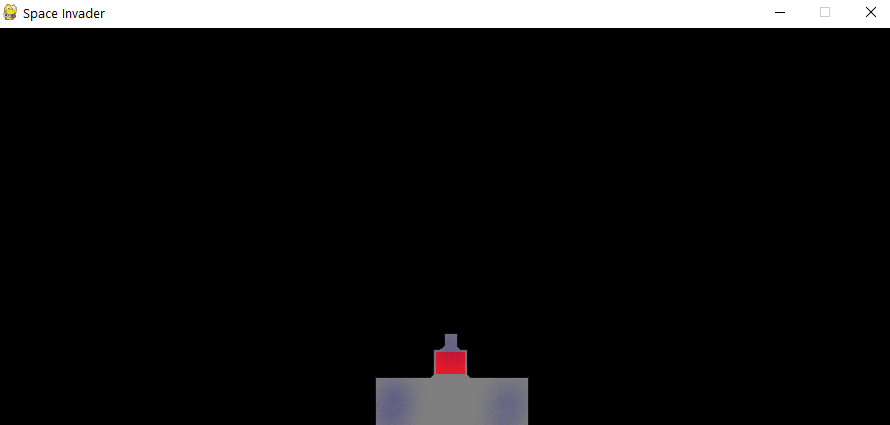
\includegraphics[width=0.7\linewidth]{validacion01.png}
    \caption{Validación de la implementación \ref{objetivo3}}
    \label{validacion01}
\end{figure}

\subsection{Sobre la implementación \ref{objetivo4}}
Como se observa en la figura \ref{validacion04}, se corrobora la funcionalidad de la implementación \ref{objetivo4}.
\begin{figure}[H]
    \centering
    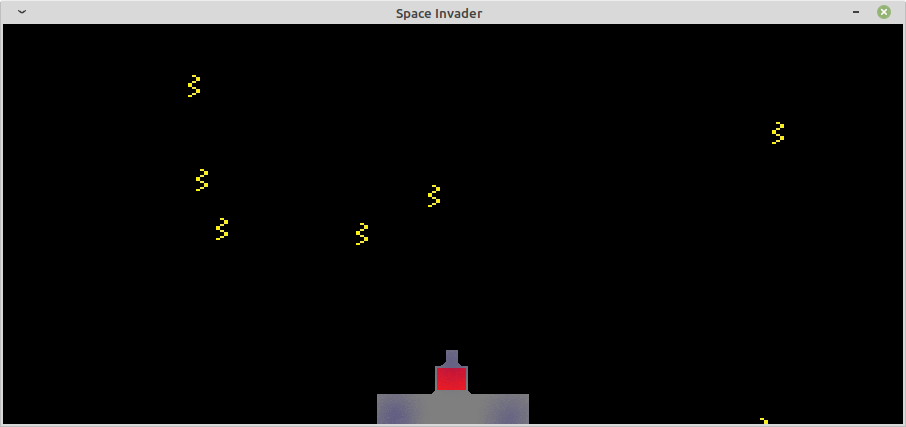
\includegraphics[width=0.7\linewidth]{jj.png}
    \caption{Validación de la implementación \ref{objetivo4}}
    \label{validacion04}
\end{figure}

\subsection{Sobre la implementación \ref{objetivo5}}
Los diferentes niveles de dificultad se validaron corriendo el juego, hay tres naves de dificultad: fácil, dos de dificultad media y una de nivel difícil. \vspace{5mm}\\
\indent A continuación se muestra la figura \ref{05}, donde se corrobora la creación de enemigos.
\begin{figure}[H]
    \centering
    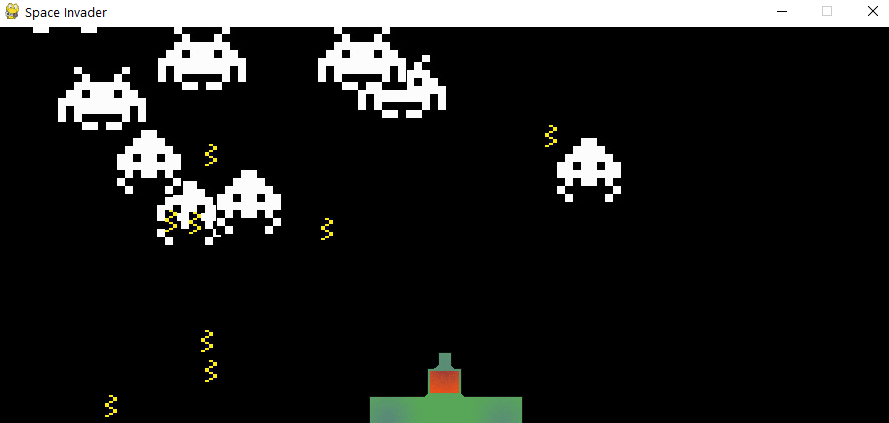
\includegraphics[width=0.7\linewidth]{validacion05.png}
    \caption{Validación de la creación de enemigos}
    \label{05}
\end{figure}
\subsection{Sobre la implementación \ref{objetivo6}}
Se validó corriendo el juego, en el cual se escuchó la música de fondo sonando y los sonidos de los disparos y las explosiones.
\subsection{Sobre la implementación \ref{objetivo7}}
Se validó corriendo el juego, en el cual visualizo la música de fondo sonando y los sonidos de selección, y sprites de elección.
\begin{figure}[H]
    \centering
    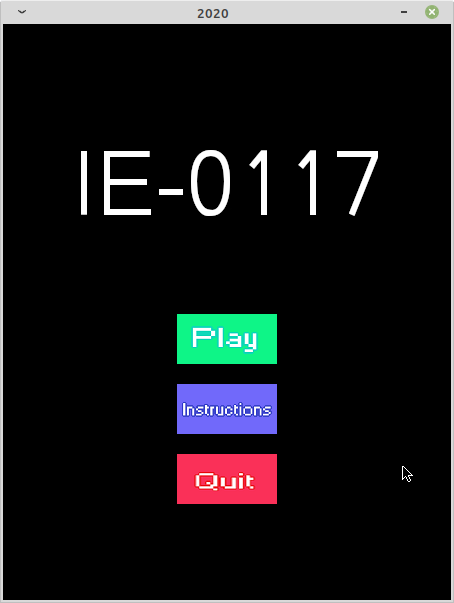
\includegraphics[width=0.7\linewidth]{Menu.png}
    \caption{Validación de la creación de menú}
    \label{05}
\end{figure}
\subsection{Sobre la implementación \ref{objetivo8}}
Se validó corriendo el juego, en el cual visualizo la pantalla final de puntaje al finalizar.
\begin{figure}[H]
    \centering
    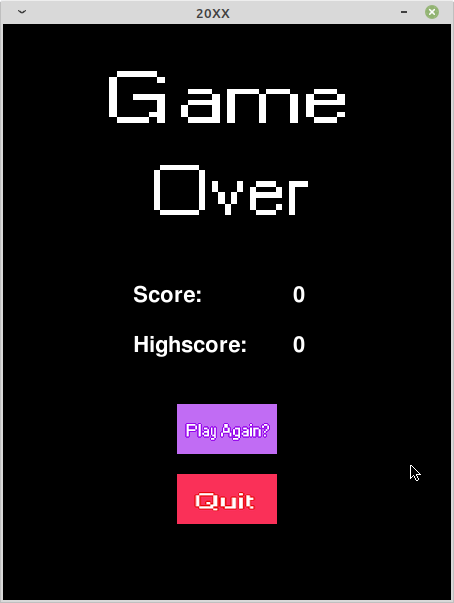
\includegraphics[width=0.7\linewidth]{score.png}
    \caption{Validación de la creación de puntaje}
    \label{05}
\end{figure}
\newpage

\section{Conclusiones}
\begin{itemize}
    \item Se logró programar un videojuego de combate de naves en 2D en lenguaje de programación \textit{Python} utilizando  \textit{Pygame}.
    \item Se seleccionó lenguage de programación Python para el videojuego. Esto porque a diferencia del lenguaje C, Python permite el uso de clases, lo cual facilita la labor de programación en casos donde se desea un enfoque de programación orientada a objetos, como en este caso. Sin embargo tiene el inconveniente de que es un poco más lento, por lo que los motores gráficos de videojuegos generalmente utilizan C++ (como el caso de Unreal Engine). C++tiene  la misma ventaja de Python de las clases y una velocidad similar a la lograda en C. Para este caso el lenguage Python funcionó adecuadamente para las condiciones deseadas y permitió programar un videojuego basándose en un enfoque de la creación de las clases Nave e Invasor. 
    \item Se pudieron añadir pistas musicales de fondo al videojuego utilizando funciones de \textit{Pygame}, particularmente \textit{pygame.mixer.music}.
    
     \item Se añadieron sonidos de disparo utilizando formato .wav con \textit{pygame.mixer.sound}. Se utilizó .wav para que no interfiriera con la música de fondo que está en formato mp3 y \textit{Pygame} solo permite reproducir un mp3 a la vez.
     
    \item Se lograron implementar otros niveles cambiando la dificultad según la nave elegida. Esto debido a no hay muchas posibilidades de variacion por el tipo de juego. 
    
    \item Dado que todo el juego se desarrolla con ayuda de Pygame, para lograr la función principal del juego, que corresponde a establecer una interfaz gráfica donde se lleva a cabo el funcionamiento del mismo, se hacen uso de distintos módulos de Pygame, tales como \texttt{sys, display}.
    
    \item Pygame está basado en una biblioteca que permite crear juegos y programas multimedia con mayor facilidad. Para la creación de los objetos en el juego, tales como la nave del jugador, se definen los atributos y las funciones del mismo con ayuda de la biblioteca que nos ofrece Pygame.
    
    \item Para la creación de enemigos y el nivel de dificultad, se crearon funciones y clases con ayuda de los módulos que ofrece Pygame. Para la funcionalidad de las mismas se tomaron en cuenta la cantidad de enemigos y el tiempo entre disparos.
    
    \item Una de las facilidades con las que se cuenta en Pygame, es que se pueden implementar archivos multimedia, por ejemplo, con ayuda del módulo pygame.mixer.music, permite controlar el audio que se le pasa como paramétro. Esto siendo utilizado para distintos sonidos en el juego, como la pista de fondo o la colisión de la nave.
\end{itemize}
\newpage
 
 \section{Recomendaciones}
 \begin{itemize}
     \item Se recomienda como trabajo futuro permitir el movimiento vertical de la nave, que en este caso se limito a la dimensión hoizontal
     \item Se deja como trabajo futuro añadir componente horizontal a la velocidad de los proyectiles, que en este caso se dejó con componente vertical únicamente
 \end{itemize}
 \newpage
\section{Bibliografía} 
\begin{enumerate}
\item Challenger-Pérez, I., Díaz-Ricardo, Y., \& Becerra-García, R. A. (2014). El lenguaje de programación Python. Ciencias Holguín, 20(2), 1-13.

\item Echeverría, M. A. (2014). Acceso Abierto y software libre. e-Ciencias de la Información, 1-11.

\item Fincher, J. (2015-2020). PyGame: A Primer on Game Programming in Python. Real Python. Recuperado de: \url{https://realpython.com/pygame-a-primer/\#background-and-setup}

\item Geeksforgeeks. (2020). Comparison of Python with other programming languages. GeeksforGeeks. Recuperado de: \url{https://www.geeksforgeeks.org/comparison-of-python-with-other-programming-languages/}

\item GitHub. (2017-). Ejemplo juego de naves en Pyhton. Recuperado de:\url{https://github.com/jerryxihe/20XX}

\item Godot Comunity. (2014-2020). Introduction. Godot Engine. Recuperado de: \url{https://godotengine.org/}

\item NumPy. (2020). What is NumPy? NumPy. Recuperado de: \url{https://numpy.org/doc/stable/user/whatisnumpy.html}

\item Python.org. (s.f). Python Documentation. Recuperado de: \url{https://wiki.python.org/moin/}

\item Python. (s.f). What is Python? Executive Summary. Python. Recuperado de: \url{https://www.python.org/doc/essays/blurb/}

\item SDL. (s.f). About SDL. Simple Directmedia Layer. Recuperado de: \url{https://www.libsdl.org/}

\end{enumerate}

\end{document}





